% XeLaTeX document
\documentclass[12pt,a4paper]{article}

% Редактируем: конфигурация, личные настройки: имя, название предмета и пр. для титульной страницы и метаданных документа здесь
\newcommand{\university}{Санкт-Петербургский политехнический университет Петра Великого}
\newcommand{\faculty}{Институт прикладной математики и механики}
\newcommand{\department}{Кафедра «Прикладная математика»}
\newcommand{\city}{Санкт-Петербург}
\newcommand{\num}{ №6}
\newcommand{\docname}{Отчёт по лабораторной работе}
\newcommand{\subject}{Математическая статистика}
\newcommand{\tutorname}{Баженов А. Н.}
\newcommand{\studentname}{Бавыкина М. А.}
\newcommand{\group}{3630102/70401}

% Не редактируем: используемые пакеты
% настройка кодировки, шрифтов и русского языка
\usepackage{fontspec}
\usepackage{polyglossia}

% рабочие ссылки в документе
\usepackage{hyperref}

% графика
\usepackage{graphicx}
\usepackage{tikz}
% поворот страницы
\usepackage{pdflscape}

% качественные листинги кода
\usepackage{minted}
\usepackage{listings}
\usepackage{lstfiracode}

% отключение копирования номеров строк из листинга, работает не во всех просмотрщиках (в Adobe Reader работает)
\usepackage{accsupp}
\newcommand\emptyaccsupp[1]{\BeginAccSupp{ActualText={}}#1\EndAccSupp{}}
\let\theHFancyVerbLine\theFancyVerbLine
\def\theFancyVerbLine{\rmfamily\tiny\emptyaccsupp{\arabic{FancyVerbLine}}}

% библиография
\bibliographystyle{templates/gost-numeric.bbx}
\usepackage{csquotes}
\usepackage[parentracker=true,backend=biber,hyperref=false,bibencoding=utf8,style=numeric-comp,language=english,autolang=other,citestyle=gost-numeric,defernumbers=true,bibstyle=gost-numeric,sorting=ntvy,]{biblatex}

% установка полей
\usepackage{geometry}

% нумерация картинок по секциям
\usepackage{chngcntr} 
\usepackage{subfigure}

% дополнительные команды для таблиц
\usepackage{booktabs}

% для заголовков
\usepackage{caption} 
\usepackage{titlesec}
\usepackage[dotinlabels]{titletoc}

% разное для математики
\usepackage{amsmath, amsfonts, amssymb, amsthm, mathtools}

% водяной знак на документе, см. main.tex
\usepackage[printwatermark]{xwatermark} 


% Не редактируем: параметры используемых пакетов и не только
% настройки polyglossia
\setdefaultlanguage{russian}
\setotherlanguage{english}

% локализация
\addto\captionsrussian{
  \renewcommand{\figurename}{Рисунок}%
  \renewcommand{\partname}{Глава}
  \renewcommand{\contentsname}{\centerline{Содержание}}
  \renewcommand{\listingscaption}{Листинг}
}

% основной шрифт документа
\setmainfont{CMU Serif}

% перечень использованных источников
\addbibresource{refs.bib}

% настройка полей
\geometry{top=2cm}
\geometry{bottom=2cm}
\geometry{left=2cm}
\geometry{right=2cm}
\geometry{bindingoffset=0cm}


% настройка ссылок и метаданных документа
\hypersetup{unicode=true,colorlinks=true,linkcolor=black,citecolor=green,filecolor=magenta,urlcolor=cyan,		       
    pdftitle={\docname},   	    
    pdfauthor={\studentname},      
    pdfsubject={\subject},      		        
    pdfcreator={\studentname}, 	       
    pdfproducer={Overleaf}, 		     
    pdfkeywords={\subject}
    }


% настройка подсветки кода и окружения для листингов
\usemintedstyle{colorful}
\newenvironment{code}{\captionsetup{type=listing}}{}

% шрифт для листингов с лигатурами
\setmonofont{FiraCode-Regular.otf}[
    Path = templates/,
    Contextuals=Alternate
]

% оформления подписи рисунка
\captionsetup[figure]{labelsep = period}

% подпись таблицы
%\DeclareCaptionFormat{hfillstart}{\hfill#1#2#3\par}
%\captionsetup[table]{format=hfillstart,labelsep=newline,justification=centering,skip=-10pt,textfont=bf}

% путь к каталогу с рисунками
\graphicspath{{fig/}}

% Внесение titlepage в учёт счётчика страниц
\makeatletter
\renewenvironment{titlepage} {
 \thispagestyle{empty}
}
\makeatother

\counterwithin{figure}{section}
\counterwithin{table}{section}

\titlelabel{\thetitle.\quad}

% для удобного конспектирования математики
%\mathtoolsset{showonlyrefs=true}
\theoremstyle{plain}
\newtheorem{theorem}{Теорема}[section]
\newtheorem{proposition}[theorem]{Утверждение}
\theoremstyle{definition}
\newtheorem{corollary}{Следствие}[theorem]
\newtheorem{problem}{Задача}[section]
\theoremstyle{remark}
\newtheorem*{nonum}{Решение}

% настоящее матожидание
\newcommand{\MExpect}{\mathsf{M}}

% объявили оператор!
\DeclareMathOperator{\sgn}{\mathop{sgn}}

% перенос знаков в формулах (по Львовскому)
\newcommand*{\hm}[1]{#1\nobreak\discretionary{} {\hbox{$\mathsurround=0pt #1$}}{}} 


% водяной знак для обозначения статуса документа
% \newwatermark[allpages,color=red!5,angle=45,scale=3,xpos=0,ypos=0]{DRAFT}
\begin{document}
% Не редактируем: Титульная страница (формируется автоматически из заданной конфигурации)
\begin{titlepage}	% начало титульной страницы

	\begin{center}		% выравнивание по центру

		\large \university \\
		\large \faculty \\
		\large \department \\[6cm]
		% название института, затем отступ 6см
		
		\huge \subject \\[0.5cm] % название работы, затем отступ 0,5см
		\large \docname \num \\[5.1cm]
		% \large Тема работы\\[5cm]

	\end{center}


	\begin{flushright} % выравнивание по правому краю
		\begin{minipage}{0.25\textwidth} % врезка в половину ширины текста
			\begin{flushleft} % выровнять её содержимое по левому краю

				\large\textbf{Работу выполнил:}\\
				\large \studentname \\
				\large {Группа:} \group \\
				
				\large \textbf{Преподаватель:}\\
				\large \tutorname

			\end{flushleft}
		\end{minipage}
	\end{flushright}
	
	\vfill % заполнить всё доступное ниже пространство

	\begin{center}
	\large \city \\
	\large \the\year % вывести дату
	\end{center} % закончить выравнивание по центру

\end{titlepage} % конец титульной страницы

\vfill % заполнить всё доступное ниже пространство


% Не редактируем: Страница содержания (формируется автоматически из section, subsection и пр., указанных в content.tex)
% Содержание
\tableofcontents
\newpage



% Редактируем: всё остальное: вступление, др. этапы, заключение, приложение
\newpage
\listoffigures

\newpage
\listoftables

\newpage
\section{Постановка задачи}
Сгенерировать двумерные выборки размерами 20, 60, 100 для нормального двумерного распределения $N(x, y, 0, 0, 1, 1, \rho)$. Коэффициент корреляции $\rho$ взять равным 0, 0.5, 0.9.
Каждая выборка генерируется 1000 раз и для неё вычисляются: среднее значение, среднее значение квадрата и дисперсия коэффициентов корреляции Пирсона, Спирмена и квадрантного коэффициента корреляции.
Повторить все вычисления для смеси нормальных распределений:
\begin{equation} \label{eq:f(x, y)}
f(x, y) = 0.9N(x, y, 0, 0, 1, 1, 0.9) + 0.1N(x, y, 0, 0, 10, 10, -0.9)
\end{equation}
Изобразить сгенерированные точки на плоскости и нарисовать эллипс
равновероятности.
\addcontentsline{toc}{section}{Постановка задачи}

\section{Теория}
\subsection{Двумерное нормальное распределение}
Двумерное нормальное распределение является частным случаем многомерного нормального распределения. Плотность вероятности двумерной случайной величины $X, Y$, распределённой нормально, выражается формулой:
\begin{equation} \label{eq:N(x, y...)} 
N(x, y, \overline{x}, \overline{y}, \sigma_x, \sigma_y, \rho) = 
\frac{1}{2 \pi \sigma_x \sigma_y \sqrt{1-\rho^2}} 
exp (-\frac{1}{2(1-\rho^2)} [\frac{(x-\overline{x})^2}{\sigma_x^2}
- 2\rho\frac{(x-\overline{x})(y-\overline{y})}{\sigma_x \sigma_y} + \frac{(y-\overline{y})^2}{\sigma_y^2}])
\end{equation}
Параметр $\rho$ называется коэффициентом корреляции.

\subsection{Корреляционный момент (ковариация) и коэффициент корреляции}
Ковариация — мера линейной зависимости двух случайных величин. Ковариация двух случайных величин $X$ и $Y$, определённых на одном и том же вероятностном пространстве, определяется формулой:
\begin{equation} \label{eq:K}
K = cov(X, Y) = M[(X-\overline{x})(Y-\overline{Y})] 
\end{equation}
Корреляция — взаимосвязь двух или более случайных величин. Математической мерой корреляции двух случайных величин $X$ и $Y$ служит коэффициент корреляции $\rho$, который определяется отношением:
\begin{equation} \label{eq:K}
\rho = \frac{K}{\sigma_x \sigma_y}
\end{equation}
Коэффициент корреляции изменяется в пределах от минус единицы до плюс единицы.

\subsection{Выборочные коэффициенты корреляции}
\subsubsection{Выборочный коэффициент корреляции Пирсона}
Естественной оценкой для $\rho = \frac{cov(X,Y)}{\sqrt{DXDY}}$ служит его статистический аналог в виде выборочного коэффициента корреляции, предложенного К.Пирсоном, —
\begin{equation} \label{eq:r}
r = \frac{1/n\sum(x_i-\overline{x})(y_i-\overline{y})} 
{1/n\sum (x_i-\overline{x})^2 1/n\sum (y_i-\overline{y})^2} 
= K/(s_Xs_Y),
\end{equation}
где $K, s^2_X, s^2_Y$ — выборочные ковариация и дисперсии с.в. $X$ и $Y$. \\ \\
Коэффициент корреляции Пирсона характеризует существование линейной зависимости между двумя величинами. Коэффициент также называют также теснотой линейной связи. \cite{theory}

\subsubsection{Выборочный квадрантный коэффициент корреляции}
Кроме выборочного коэффициента корреляции Пирсона, существуют и другие оценки степени взаимосвязи между случайными величинами. К ним относится выборочный квадрантный коэффициент корреляции 
\begin{equation} \label{eq:r}
r_Q = \frac{(n_1+n_3)-(n_2+n_4)} 
{n},
\end{equation}
где $n_1, n_2, n_3, n_4$ — количества точек с координатами $(x_i, y_i)$, попавшими соответственно в I, II, III и IV квадранты декартовой системы с осями $x^{'} = x -  med x, y^{'} = y -  med y$ и с центром в точке с координатами $(med x, med y)$. \cite{theory}


\subsubsection{Выборочный коэффициент ранговой корреляции Спирмена}
Если требуется оценить степень взаимодействия между качественными признаками изучаемого объекта, для оценки силы связи используются не численные значения, а соответствующие им ранги. Сам процесс упорядочения называется ранжированием.\\ \\
Если объект обладает не одним, а двумя качественными признаками — переменными $X, Y$, то для исследования их взаимосвязи используют выборочный коэффициент корреляции между двумя последовательностями рангов этих признаков. \\ \\
Обозначим ранги, соотвествующие значениям переменной $X$, через $u$, а ранги, соотвествующие значениям переменной $Y$ — через $v$. Выборочный коэффициент ранговой корреляции Спирмена определяется как выборочный коэффициент корреляции Пирсона между рангами $u, v$ переменных $X, Y$:
\begin{equation} \label{eq:r_S}
r_S = \frac{1/n\sum(u_i-\overline{u})(v_i-\overline{v})} 
{\sqrt{1/n\sum (u_i-\overline{u})^2 1/n\sum (v_i-\overline{v})^2}},
\end{equation}
где $\overline{u} = \overline{v} = \frac{1 + 2 + ... + n}{n} = \frac{n+1}{2}$ — среднее значение рангов. \cite{theory}

\subsection{Эллипсы рассеивания}
Поверхность распределения, изображающую данную функцию, имеет вид холма, вершина которого находится над точкой $(\overline{x}, \overline{y})$. В сечении поверхности распределения плоскостями, параллельными плоскости $xOy$ получаются эллипсы. \cite{ellipse_theory} Уравнение проекции такого эллипса на плоскость $xOy$:
\begin{equation} \label{eq:const}
\frac{(x-\overline{x})^2}{\sigma_x^2}
- 2\rho\frac{(x-\overline{x})(y-\overline{y})}{\sigma_x \sigma_y} + \frac{(y-\overline{y})^2}{\sigma_y^2} = const
\end{equation}
Осей симметрии эллипса составляют с осью  $Ox$ углы, определяемые уравнением
\begin{equation} \label{eq:const}
tg 2\alpha = \frac{2\rho\sigma_x\sigma_y}{\sigma_x^2 - \sigma_y^2} 
\end{equation} 
Во всех точках каждого из таких эллипсов плотность распределения $N(x, y, \overline{x}, \overline{y}, \sigma_x, \sigma_y, \rho)$ постоянна. Поэтому такие эллипсы называются называется эллипсами равной плотности, ограниченная ими область – эллипсами рассеивания, центры эллипсов – центрами рассеивания.


\section{Реализация}
Лабораторная работа была выполнена с помощью встроенных средств языка программирования Python в среде разработки IDLE. Исходный код лабораторной работы приведён по ссылке. В ходе работы использовались библиотеки Math, Matplotlib, Numpy и Seaborn. \\ \\
Помимо основных в ходе работы были использованы следующие инструменты:
\begin{itemize}
\item $multivariate.normal$ : генерация двумерных выборк размерами 20, 60, 100 для нормального двумерного распределения \cite{ellipse}
\item stats.pearsonr : вычисление коэффициента корреляции Пирсона
\item stats.spearmanr:  вычисление коэффициента корреляции Спирмена
\item $confidence.ellipse$ : построение эллипсов рассеивания
\end{itemize}

\section{Результаты}
\subsection{Выборочные коэффициенты корреляции}

\begin{table} [h]
\begin{center}
\begin{tabular}{|c|c|}
	\hline
	$Номер результата измерений j$ & $Результат измерений x_j$\\
	\hline
	1 & 15.61 \\ 
	\hline
	2 & 20.71 \\ 
	\hline
	3 & 21.68 \\ 
	\hline
	4 & 22.28 \\ 
	\hline
	5 & 23.22 \\ 
	\hline
	6 & 24.14 \\ 
	\hline
	7 & 24.59 \\ 
	\hline
	8 & 26.18 \\ 
	\hline
	9 & 26.23 \\ 
	\hline
	10 & 27.59 \\ 
	\hline
	11 & 27.88 \\ 
	\hline
	12 & 28.74 \\ 
	\hline
	13 & 29.34 \\ 
	\hline
	14 & 30.86 \\ 
	\hline
	15 & 32.08 \\ 
	\hline
\end{tabular}
\end{center}
\caption{Результаты измерений, упорядоченные по значению, n = 15}
\end{table} 

\begin{figure}[h]
\center{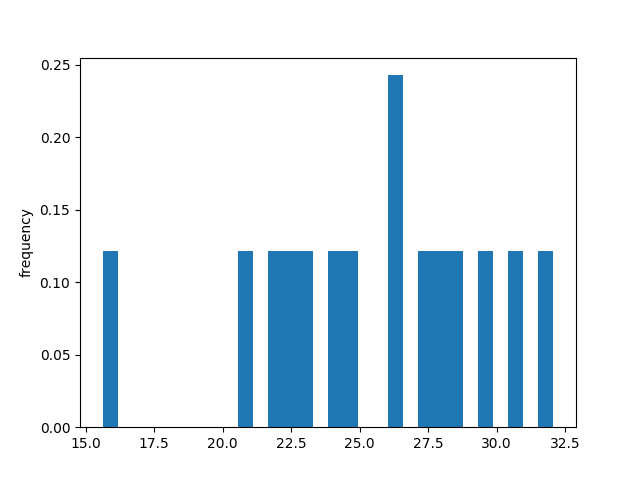
\includegraphics[width=1\linewidth]{normCramer.png}}
\caption{Пробная выборка, n = 15}
\label{fig:box20}
\end{figure}


\begin{table} [h]
\resizebox{0.7\textwidth}{!}{\begin{minipage}{\textwidth}
\begin{tabular}{|c|c|c|c|c|c|c|c|c|c|}
	\hline
	$j$ & $A_j=\frac{2j-1}{2n}$ & $B_j=F(x_j)$  & $C_j=ln(B_j)$ & $D_j=(A_j)(C_j)$ & $E_j=1-A_j$ & $F_j=1-B_j$ & $G_j=ln(F_j))$ & $H_j=(E_j)(G_j)$ & $I_j=(D_j)+(H_j)$\\
	\hline
	 1 & 0.033 &  0.011723  & -4.44618 &  -0.14820 &  0.9666 &  0.988277 & -0.01179  & -0.01139 & -0.1596\\
	 \hline
	 2 &  0.100 &  0.138600   & -1.97616 &  -0.19761 &  0.9000 &  0.861400 & -0.14919  & -0.13427 & -0.33189\\
	 \hline
	 3 &  0.167 &  0.194259   &  -1.63856 & -0.27309 &  0.8333 &  0.805741 & -0.21599  & -0.17999 & -0.45308\\
	 \hline
	 4 & 0.233  &  0.234672  &  -1.44956 &  -0.33823 &  0.7666 &  0.765328 & -0.26745  & -0.20504 & -0.54327\\
	 \hline
	 5 & 0.300 &  0.306372   &  -1.18295 &  -0.35488 &  0.7000 &  0.693628 & -0.36582  & -0.25607 & -0.61096\\
	 \hline
	 6 & 0.367  &  0.384609   &  -0.95552 &  -0.35036 &  0.6333 &  0.615391 & -0.48549  & -0.30748 & -0.65784\\
	 \hline
	 7 & 0.433  &  0.424918  & -0.85586 &  -0.37087 &  0.5666 &  0.575082 & -0.55324  & -0.31350 & -0.68437\\
	 \hline
	 8 & 0.500 &  0.570788  & -0.56073 & -0.28036 &  0.5000 &  0.429212 & -0.84580  & -0.42290 & -0.70327\\
	 \hline
	 9 & 0.567  & 0.575324   &  -0.55282 &  -0.31326 &  0.4333 &  0.424676 & -0.85642  & -0.37111 & -0.68438\\
	 \hline
	 10 & 0.633  &  0.693032  &  -0.36667 &  -0.23223 &  0.3666 &  0.306968 & -1.18101  & -0.43303 & -0.66526\\
	 \hline
	 11 &  0.700  & 0.716180   &  -0.33382 &  -0.23367 &  0.3000 &  0.283820 & -1.25941  & -0.37782 & -0.61150\\
	 \hline
	 12 & 0.767  &  0.779474   &  -0.24913 &  -0.19100 &  0.2333 &  0.220526 & -1.51174  & -0.35273 & -0.54374\\
	 \hline
	 13 & 0.833  &  0.818371   &  -0.20043 &  -0.16703 &  0.1666 &  0.181629 & -1.70579  & -0.28429 & -0.45133\\
	 \hline
	 14 & 0.900  &  0.896291   &  -0.10949 &  -0.09854 &  0.1000 &  0.103709 & -2.26616 & -0.22661 & -0.32515\\
	 \hline
	 15 & 0.967  &  0.938565  &  -0.06340 &  -0.06129 &  0.0333 &  0.061435 & -2.78977 &  -0.09299 & -0.15428\\
	\hline
	$\sum$ & & & & & & & & & -7.57998\\
	\hline
\end{tabular}
\end{minipage} }
\caption{Результаты промежуточных вычислений значения статистики $n\Omega_n^2$ по формуле \ref{eq:Г1}, n = 15} \label{tab:nomega} 
\end{table} 








\begin{table} [h]
\begin{center}
\begin{tabular}{|c|c|}
	\hline
	$Номер результата измерений j$ & $Результат измерений x_j$\\
	\hline
	1 & -2.46 \\ \hline
2 & -2.10 \\ \hline
3 & -1.16 \\ \hline
4 & -1.04 \\ \hline
5 & -0.99 \\ \hline
6 & -0.92 \\ \hline
7 & -0.91 \\ \hline
8 & -0.71 \\ \hline
9 & -0.66 \\ \hline
10 & -0.38 \\ \hline
11 & -0.27 \\ \hline
12 & -0.22 \\ \hline
13 & -0.18 \\ \hline
14 & -0.09 \\ \hline
15 & -0.06 \\ \hline
16 & 0.01 \\ \hline
17 & 0.082 \\ \hline
18 & 0.10 \\ \hline
19 & 0.16 \\ \hline
20 & 0.22 \\ \hline
21 & 0.32 \\ \hline
22 & 0.37 \\ \hline
23 & 0.43 \\ \hline
24 & 0.45 \\ \hline
25 & 0.52 \\ \hline
26 & 0.63 \\ \hline
27 & 0.76 \\ \hline
28 & 1.83 \\ \hline
29 & 1.97 \\ \hline
30 & 2.44 \\ \hline
\end{tabular}
\end{center}
\caption{Результаты измерений, упорядоченные по значению, n = 30}
\end{table} 

\begin{figure}[h]
\center{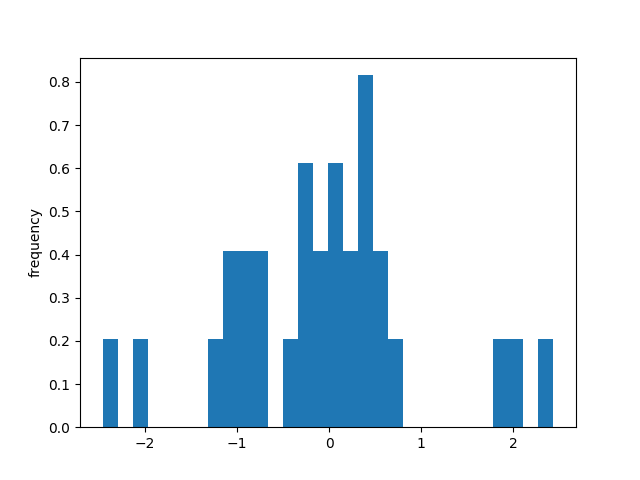
\includegraphics[width=1\linewidth]{normCramer30.png}}
\caption{Пробная выборка, n = 30}
\label{fig:box20}
\end{figure}


\begin{table} [h]
\resizebox{0.7\textwidth}{!}{\begin{minipage}{\textwidth}
\begin{tabular}{|c|c|c|c|c|c|c|c|c|c|}
	\hline
	$j$ & $A_j=\frac{2j-1}{2n}$ & $B_j=F(x_j)$  & $C_j=ln(B_j)$ & $D_j=(A_j)(C_j)$ & $E_j=1-A_j$ & $F_j=1-B_j$ & $G_j=ln(F_j))$ & $H_j=(E_j)(G_j)$ & $I_j=(D_j)+(H_j)$\\
	\hline
	 1 &  0.017 &  0.011222 &  -4.48988 &  -0.07483 &  0.9833 &  0.988778 &  -0.01129 &  -0.01110 &  -0.08593 \\ \hline
2 &  0.050 &  0.025776 &  -3.65829 &  -0.18291 &  0.9500 &  0.974224 &  -0.02611 &  -0.02481 &  -0.20772 \\ \hline
3 &  0.083 &  0.146270 &  -1.92230 &  -0.16019 &  0.9167 &  0.853730 &  -0.15814 &  -0.14496 &  -0.30515 \\ \hline
4 &  0.117 &  0.175266 &  -1.74145 &  -0.20317 &  0.8833 &  0.824734 &  -0.19269 &  -0.17021 &  -0.37338 \\ \hline
5 &  0.150 &  0.187294 &  -1.67507 &  -0.25126 &  0.8500 &  0.812706 &  -0.20739 &  -0.17628 &  -0.42754 \\ \hline
6 &  0.183 &  0.205472 &  -1.58245 &  -0.29012 &  0.8167 &  0.794528 &  -0.23001 &  -0.18784 &  -0.47795 \\ \hline
7 &  0.217 &  0.209139 &  -1.56476 &  -0.33903 &  0.7833 &  0.790861 &  -0.23463 &  -0.18380 &  -0.52283 \\ \hline
8 &  0.250 &  0.268296 &  -1.31566 &  -0.32892 &  0.7500 &  0.731704 &  -0.31238 &  -0.23428 &  -0.56320 \\ \hline
9 &  0.283 &  0.282907 &  -1.26264 &  -0.35775 &  0.7167 &  0.717093 &  -0.33255 &  -0.23833 &  -0.59607 \\ \hline
10 &  0.317 &  0.378800 &  -0.97075 &  -0.30740 &  0.6833 &  0.621200 &  -0.47610 &  -0.32534 &  -0.63274 \\ \hline
11 &  0.350 &  0.419482 &  -0.86873 &  -0.30406 &  0.6500 &  0.580518 &  -0.54384 &  -0.35349 &  -0.65755 \\ \hline
12 &  0.383 &  0.439694 &  -0.82168 &  -0.31498 &  0.6167 &  0.560306 &  -0.57927 &  -0.35722 &  -0.67219 \\ \hline
13 &  0.417 &  0.452555 &  -0.79285 &  -0.33035 &  0.5833 &  0.547445 &  -0.60249 &  -0.35145 &  -0.68181 \\ \hline
14 &  0.450 &  0.487318 &  -0.71884 &  -0.32348 &  0.5500 &  0.512682 &  -0.66810 &  -0.36745 &  -0.69093 \\ \hline
15 &  0.483 &  0.497777 &  -0.69760 &  -0.33717 &  0.5167 &  0.502223 &  -0.68871 &  -0.35583 &  -0.69301 \\ \hline
16 &  0.517 &  0.524544 &  -0.64523 &  -0.33337 &  0.4833 &  0.475456 &  -0.74348 &  -0.35935 &  -0.69272 \\ \hline
17 &  0.550 &  0.557874 &  -0.58362 &  -0.32099 &  0.4500 &  0.442126 &  -0.81616 &  -0.36727 &  -0.68826 \\ \hline
18 &  0.583 &  0.565397 &  -0.57023 &  -0.33263 &  0.4167 &  0.434603 &  -0.83332 &  -0.34722 &  -0.67985 \\ \hline
19 &  0.617 &  0.586767 &  -0.53313 &  -0.32876 &  0.3833 &  0.413233 &  -0.88374 &  -0.33877 &  -0.66753 \\ \hline
20 &  0.650 &  0.606438 &  -0.50015 &  -0.32510 &  0.3500 &  0.393562 &  -0.93252 &  -0.32638 &  -0.65148 \\ \hline
21 &  0.683 &  0.644371 &  -0.43948 &  -0.30031 &  0.3167 &  0.355629 &  -1.03387 &  -0.32739 &  -0.62770 \\ \hline
22 &  0.717 &  0.662093 &  -0.41235 &  -0.29552 &  0.2833 &  0.337907 &  -1.08499 &  -0.30741 &  -0.60293 \\ \hline
23 &  0.750 &  0.680732 &  -0.38459 &  -0.28844 &  0.2500 &  0.319268 &  -1.14173 &  -0.28543 &  -0.57387 \\ \hline
24 &  0.783 &  0.687730 &  -0.37436 &  -0.29325 &  0.2167 &  0.312270 &  -1.16389 &  -0.25218 &  -0.54542 \\ \hline
25 &  0.817 &  0.712201 &  -0.33940 &  -0.27717 &  0.1833 &  0.287799 &  -1.24549 &  -0.22834 &  -0.50551 \\ \hline
26 &  0.850 &  0.747836 &  -0.29057 &  -0.24699 &  0.1500 &  0.252164 &  -1.37767 &  -0.20665 &  -0.45364 \\ \hline
27 &  0.883 &  0.784050 &  -0.24328 &  -0.21490 &  0.1167 &  0.215950 &  -1.53271 &  -0.17882 &  -0.39372 \\ \hline
28 &  0.917 &  0.964333 &  -0.03632 &  -0.03329 &  0.0833 &  0.035667 &  -3.33352 &  -0.27779 &  -0.31109 \\ \hline
29 &  0.950 &  0.973784 &  -0.02657 &  -0.02524 &  0.0500 &  0.026216 &  -3.64139 &  -0.18207 &  -0.20731 \\ \hline
30 &  0.983 &  0.991406 &  -0.00863 &  -0.00849 &  0.0167 &  0.008594 &  -4.75673 &  -0.07928 &  -0.08777 \\ \hline
	$\sum$ & & & & & & & & & -15.2768\\
	\hline
\end{tabular}
\end{minipage} }
\caption{Результаты промежуточных вычислений значения статистики $n\Omega_n^2$ по формуле \ref{eq:Г1}, n = 30} \label{tab:nomega} 
\end{table} 
\section{Обсуждение}
Гипотеза $H_0$ о нормальном законе распределения $N(x, \hat{\mu}, \hat{\sigma})$ при уровне значимости $\alpha = 0.2$ согласуется с выборкой.

\section{Приложение}
Исходный код текста программ можно найти по ссылке \\ https://github.com/mariiabav/MathStatistics.git   

% Не редактируем: Страница библиографии (формируется автоматически из книжек, указанных в refs.bib и пометок \cite{имя_источника} в тексте)
\newpage
\printbibliography[title=Перечень использованных источников]
\addcontentsline{toc}{section}{Перечень использованных источников}
\end{document}
